This section will include the simulation and programming part of the work, experimental part

\section{Simulation of bubble response}

\section{Experiment of measuring bubbles}


\begin{center}
	\begin{tabular}{l r}
		Date Performed: & May 17, 2024 \\ % Date the experiment was performed
		Partners: & Viktoriia \textsc{Boichenko} \\
		Instructor: & Christian \textsc{Kanarski} % Instructor/supervisor
	\end{tabular}
\end{center}

% If you need to include an abstract, uncomment the lines below
%\begin{abstract}
%	Abstract text
%\end{abstract}

%----------------------------------------------------------------------------------------
%	OBJECTIVE
%----------------------------------------------------------------------------------------

\section{Objective}

This laboratory project aims to connect theoretical concepts with empirical observations through the use of volume strength backscattering. The primary objective is to illustrate the practical applications of theoretical knowledge acquired during the internship and master’s thesis research. 

By leveraging volume strength backscattering as a key analytical tool, we will examine experimental data, providing insights into how theoretical abstractions translate into concrete experimental methodologies. This integration is designed to promote a comprehensive understanding of the reciprocal relationship between theory and practice, underscoring the significance of a multidimensional approach in scientific inquiry and engineering practice.

\begin{description}
	\item[Sonars] 

    The general principle of the projector SIMO-sonar is in the following way:  the signal is emitted with a single transducer and receiving a signal back with several receivers, which in our case were hydrophones. Also, it can be considered with another interpretation. For example, we provide a single output, and obtain multiple input data.
    
    The sonar type is the SIMO-sonar, as we needed to start with a simple model of the current research. The experiments with a MIMO-sonar can be implemented for further research therefore expanding the complexity and variability of usages of the developed model, as [this type provides an improved resolution and enhances the signal-to-noise ratio of the received signal] (http://jset.sasapublications.com/wp-content/uploads/2017/09/6702529.pdf).
    
	\item[Bubble flare] 

    A continuous column of bubbles with the different radii which is emitted with a bubble generator. Minimum bubble size that the machine could produce were 
	\item[] 
    
    %or whatever definition you want to add 
\end{description} 

\section{Experimental model}

The experimental setup entails an experiment of bubbles flares detection with a sonar. They were emitted in a water with a bubble generator and observed with the help of the SIMO-sonar with an ultrasound in a laboratory conditions of the water tank. 

Preliminary tests of the water tank were performed in order to identify the impulse response of the  environment, and verify the correctness of the equipment configuration as well as whether it is in a usable condition.

The primary focus of the observation was the volume strength back scattering (Vs), chosen as the key parameter for assessing the acoustic bubble response with acoustic radiation in the high-frequency range. 

\section{ The setup}

Our bubble experiment was conducted using a meticulously designed setup aimed at exploring the acoustic frequency response of the bubbles. The experimental arrangement included the following:
\begin{itemize}
    \item \textbf{Bubble generator}: a set of the equipment which included
    \item \textbf{Sonar} it is a projector with 32 hydrophones in an array. The distance between elements is 0.0139 m.
    \item \textbf{Laptop with a processing software KiRAT, contains an inbuilt wave generator}
    \item \textbf{Videocamera}: a mobilephone's camera was used for the experiment recordings
\end{itemize}

During the experiment different signal types (noise and chirp) and length (2 ms and 10 ms) were used for the analysis of the bubble flares. The emitted central frequency was 50 kHz with a bandwidth of 40 kHz. The sampling frequency was 192 kHz.
\begin{itemize}
    \item \textbf{Noise}: a white noise whose frequency is not dependent on the power spectral density\cite*{ainslie_principles_2010};  
    \item \textbf{Chirp}: a hyperbolic frequency modulation upward signal 
\end{itemize}

\begin{itemize}
    \item  Sound signal: narrow band pulse, chirp, noise
    \item Sonar position: from top, vertical, horizontal
    \item Bubbles location: in the center of the experimental pool
   \item Bubble characteristics: emitting a single bubble of the specified radius; a row of bubbles; 
   creating a bubble flare;
\end{itemize}
Other things which are important for taking into account are:
\begin{itemize}
    \item Response of the transducer can influence the received signal
    \item Near field radiation implementation for measurements with a spherical radiation against the plane wave in a far field
\end{itemize}

Further set of things which are required to perform the experiment are the setup of the equipment required for performing our measurements. 
Essentially, it will include the sonar, a bubble generator, processing unit as a laptop/computer.

There different papers which have conducted similar experiments on bubble investigation. 

The Zhang et al. 2021\cite{zhang_experimental_2021} paper contains description of the experiment for investigation bubble oscillations. In order to produce cavitaion bubbles the setup used a deionised water.

In order to detect the acoustic radiation released by cavitation bubbles a fiber optic hydrophone was employed, which was calibrated and attached to oscilloscope.  
Among possible things that could affect results were the cleanliness of sensor connector, water quality and wall reflection of the shock wave.

Leblond paper provides a scheme of the vertical and horizontal observation of the acoustic bubble release\cite{leblond_acoustic_2014}. Vertical will allow to detect bubbles all along the acoustic beam, while for horizontal we will see only the crossing of the stream.

\section{Experimental Data}


After the pocessing the date of 23 recorded measurements, a few results as well as comparisons can be presented below. 

At the horizontal orientation samples 8 (noise, 10ms) and 11 (chirp, 10ms).

At the vertical orientation sample 19 (noise) and 23 (chirp, 10ms) are seem to be good for comparison.

\textbf{$H_{wall}$} can be extracted from the initial measurement, calculating an impulse response of the water tank and identifying the location of the walls with the sonar.

\begin{figure}[H]
    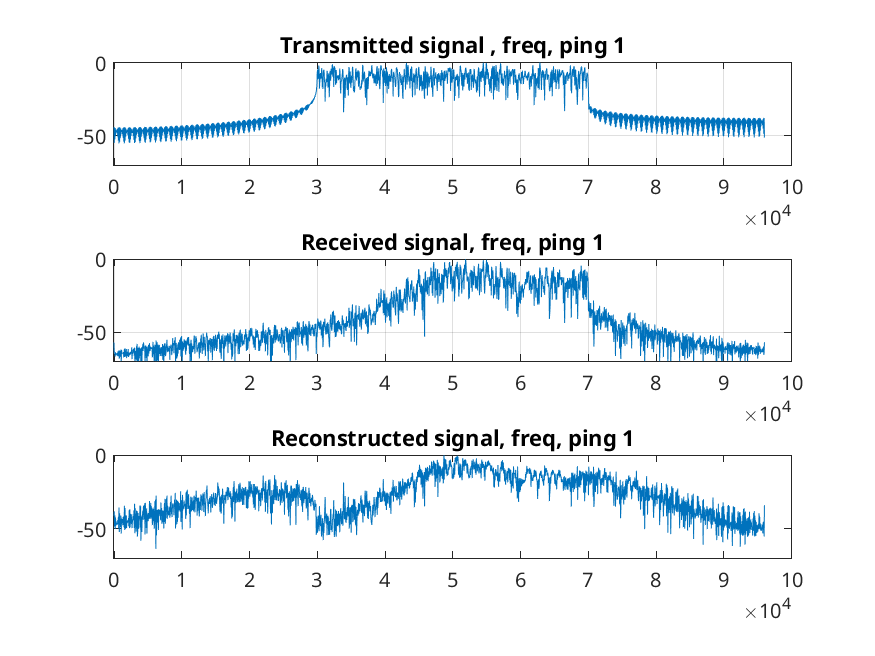
\includegraphics[width=0.7\textwidth]{reconstruction8_ping_001.png}
    \centering
    \caption*{'Horizontal orientation of the sonar, 10ms noise, sample 8'}
    \label{fig:H_noise_10ms_plot}
\end{figure}

%----------------------------------------------------------------------------------------
%	SAMPLE CALCULATION
%----------------------------------------------------------------------------------------

\section{Calculations}

\begin{itemize}
    \item Vs from a single ping
    \item spectrogram in Audacity for different samples
    \item bubble localization?
    \item obtaining $H_{bubble}$, $H_{wall}$
\end{itemize}

%----------------------------------------------------------------------------------------
%	RESULTS AND CONCLUSIONS
%----------------------------------------------------------------------------------------

\subsection{Results and Conclusions}


%----------------------------------------------------------------------------------------
%	DISCUSSION
%----------------------------------------------------------------------------------------

\subsection{Discussion of Experimental Uncertainty}

% The accepted value (periodic table) is \SI{24.3}{\gram\per\mole} \autocite{Smith:2022qr}. The percentage discrepancy between the accepted value and the result obtained here is 1.3\%. Because only a single measurement was made, it is not possible to calculate an estimated standard deviation (see \textcite{Smith:2021jd}).

% The most obvious source of experimental uncertainty is the limited precision of the balance. Other potential sources of experimental uncertainty are: the reaction might not be complete; if not enough time was allowed for total oxidation, less than complete oxidation of the magnesium might have, in part, reacted with nitrogen in the air (incorrect reaction); the magnesium oxide might have absorbed water from the air, and thus weigh ``too much." Because the result obtained is close to the accepted value it is possible that some of these experimental uncertainties have fortuitously cancelled one another.

